\documentclass{article}
\usepackage[utf8]{inputenc}
\usepackage{graphicx}
\usepackage{listings}

\title{DatabaseApex2}
\author{itsmeakil707 }
\date{November 2019}

\begin{document}

\title{CSV Python}
\author{Akil Munawwar \\ D4 TI 1B \\ 1184041}
\maketitle

\section{CSV Teori}
\subsection{Pengertian}
\paragraph{}
CSV merupakan format basis data sederhana, yang setiap record nya dipisahkan dengan tanda koma atau titik koma. Dalam python, csv sendiri sudah ada modulnya yang diciptakan untuk mempermudah mengelola data csv tersebut. Contoh file csv seperti ini.
\lstinputlisting[firstline=1, lastline=4]{src/data.csv}
\subsection{Aplikasi untuk membuat CSV}
\begin{enumerate}
    \item Editor Teks (Notepad++, Sublime, Spyder, etc)
    \item Spreadsheet (Microsoft Excel, Google Spreadshare, etc)
\end{enumerate}
\subsection{Cara membuat file CSV}
\begin{enumerate}
    \item Pertama pastikan anda mempunyai Microsoft Excel
    \item Jika sudah, jangan lupa membuat file nya seperti dibawah ini
    \begin{figure}[!htbp]
        \centering
        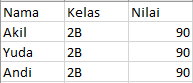
\includegraphics{figure/csv.PNG}
        \caption{Data yang akan di buat}
    \end{figure}
\newpage
    \item Jika sudah jangan lupa disimpan atau di export ke file csv
    \item Jika ingin melihat file csv tadi, tidak perlu capek membuka excel lagi, hanya buka di notepad saja sudah terbaca
    \begin{figure}[!htbp]
        \centering
        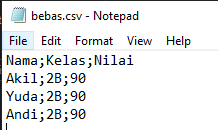
\includegraphics{figure/liatcsv.PNG}
        \caption{File CSV}
    \end{figure}
\end{enumerate}
\subsection{Sejarah library CSV}
\paragraph{}
CSV adalah format yang sering digunakan untuk export atau import database. Format CSV digunakan bertahun-tahun untuk mendekripsikan sebuah format standar pada RFC4180. Modul csv mengimplementasikan kelas untuk membaca dan menulis data tabular dalam format CSV. Hal ini memungkinkan programmer untuk mengatakan, "tulis data ini dalam format yang disukai oleh Excel," atau "baca data dari file ini yang dihasilkan oleh Excel," tanpa mengetahui detail yang tepat dari format CSV yang digunakan oleh Excel. Programmer juga dapat menggambarkan format CSV yang dipahami oleh aplikasi lain atau menentukan format CSV tujuan khusus mereka sendiri.
\newpage
\subsection{Sejarah library Pandas}
\paragraph{}
Pandas adalah librari analisis data yang memiliki struktur data yang kita perlukan untuk membersihkan data mentah ke dalam sebuah bentuk yang cocok untuk analisis (yaitu tabel). Penting untuk dicatat di sini bahwa karena pandas melakukan tugas penting seperti menyelaraskan data untuk perbandingan dan penggabungan set data, penanganan data yang hilang, dll, itu telah menjadi sebuah librari de facto untuk pemrosesan data tingkat tinggi dalam Python (yaitu statistik).
\subsection{Fungsi yang ada pada library CSV}
\begin{enumerate}
    \item csv.reader() berfungsi untuk membaca file csv
    \item csv.writer() berfungsi untuk memanipulasi file csv tersebut
\end{enumerate}
\subsection{Fungsi yang ada pada library Pandas}
\begin{enumerate}
    \item pandas.Series(data,index,dtype,copy) merupakan sebuah array satu dimensi yang memiliki label dan digunakan untuk menyimpan beragam tipe data seperti integer, string, float, bahkan objek, dan lain sebagainya. Label pada series disebut dengan index
    \item pandas.read-csv adalah fungsi yang digunakan untuk membaca file CSV
    \item pandas.to-csv adalah fungsi yang digunakan untuk menulis file berformat CSV
\end{enumerate}
\newpage
\section{Keterampilan Pemrograman}
\begin{enumerate}
    \item No 1
    \lstinputlisting[firstline=8, lastline=15]{src/1184041csv.py}
    \item No 2
    \lstinputlisting[firstline=17, lastline=22]{src/1184041csv.py}
    \item No 3
    \lstinputlisting[firstline=8, lastline=13]{src/1184041pandas.py}
    \item No 4
    \lstinputlisting[firstline=15, lastline=19]{src/1184041pandas.py}
    \item No 5
    \lstinputlisting[firstline=21, lastline=24]{src/1184041pandas.py}
\newpage
    \item No 6
    \lstinputlisting[firstline=26, lastline=30]{src/1184041pandas.py}
    \item No 7
    \lstinputlisting[firstline=32, lastline=34]{src/1184041pandas.py}
    \item No 8
    \lstinputlisting[firstline=8, lastline=11]{src/main.py}
    \item No 9
    \lstinputlisting[firstline=8, lastline=14]{src/mainpandas.py}
    \item Try Except
    \lstinputlisting[firstline=8, lastline=22]{src/try.py}
\end{enumerate}{}
\end{document}
